\documentclass[10pt,a4paper]{article}
\usepackage[utf8]{inputenc}
\usepackage[T1]{fontenc}
\usepackage{amsmath}
\usepackage{amssymb}
\usepackage{graphicx}
\usepackage{hyperref}
\usepackage{float}
\usepackage{subcaption}
\usepackage{geometry}
\geometry{a4paper, margin=1in}

\title{Investigating the Platonic Representation Hypothesis}
\author{Aryasomayajula Ram Bharadwaj\\
Independent Researcher\\
\texttt{ram.bharadwaj.arya@gmail.com}}
\date{20th Oct 2024}

\begin{document}

\maketitle

\begin{abstract}
The Platonic Representation Hypothesis (PRH) \cite{huh2024prh} suggests that neural networks, despite being trained on different objectives and datasets, converge toward a shared statistical model of reality. This work extends the investigation of PRH by exploring how neural networks behave when exposed to data that diverges from their training distribution. Using ImageNet-O as a benchmark for out-of-distribution (OOD) data, random noise as a boundary case, and detailed analyses of model alignment dynamics, we aim to uncover the strengths and limitations of PRH. Our results indicate that PRH holds in OOD contexts but encounters challenges with random data, offering a nuanced perspective on representational alignment.
\end{abstract}

\section{Introduction}
Understanding how neural networks form internal representations of the world has been a key area of research, bridging both philosophy and machine learning. The Platonic Representation Hypothesis (PRH) \cite{huh2024prh}, inspired by Plato’s Allegory of the Cave, posits that models across different domains—be it vision or language—are converging towards a shared, idealized model of reality. This hypothesis suggests that, even when trained on different datasets, models internalize similar structures, akin to Plato’s concept of perceiving shadows of the same underlying reality.

However, an important question remains: does this convergence persist when models are exposed to data significantly different from their training distributions? In this study, we address this by evaluating the behavior of PRH in various scenarios, including exposure to out-of-distribution (OOD) data and purely random data. Additionally, we explore how models' alignment evolves when progressively corrupted with noise and during different stages of language model training.

\textit{[Placeholder: Briefly introduce any philosophical or theoretical motivations specific to your study that differ from prior works.]}

\section{Methodology}
To rigorously evaluate the PRH, we designed a series of experiments that progressively test the hypothesis under varying conditions of data distribution. The methodology is structured around three main experimental setups, each focusing on a distinct aspect of model alignment.

\subsection{Experimental Setup}
\textbf{1. Representational Alignment Across Data Types:} We assessed the alignment between different models using the following datasets:
\begin{enumerate}
    \item \textbf{In-distribution data}: Places365’s validation set, which closely aligns with the training data of many vision models.
    \item \textbf{Out-of-distribution data}: The ImageNet-O dataset, specifically curated with images that fall outside the standard ImageNet distribution \cite{hendrycks2021nae}. This allows us to examine whether PRH extends to data with significant divergence.
    \item \textbf{Random noise}: A dataset of purely random images was used to probe the extreme boundaries of representational alignment. This helps determine if the models converge on a shared interpretation even when presented with unstructured input.
\end{enumerate}

We measured alignment using Spearman's rank correlation on mutual k-NN distances between model representations, comparing how models interpret the similarity of various input data points.

\textit{[Placeholder: Please describe the motivation behind using these specific datasets in more detail. Why were these choices made over others?]}

\subsection{Noise Injection in Vision Models}
\textbf{2. Progressive Noise Injection:} To understand the resilience of model alignment to data corruption, we conducted a noise injection experiment:
\begin{itemize}
    \item A set of 250 images was selected and progressively corrupted with Gaussian noise over 100 steps.
    \item At each noise level, we measured mutual alignment across 17 Vision Transformer models, evaluating how the models' representational structures changed as noise increased.
    \item The alignment scores were analyzed to reveal potential patterns in how noise impacts convergence, with a particular focus on detecting non-linear relationships.
\end{itemize}

\textit{[Placeholder: Detail the noise injection process. What type of noise was used? How were the levels of noise quantified? What criteria were used for choosing the 250 images?]}

\subsection{Tracking Alignment During Language Model Training}
\textbf{3. Evolution of Alignment During Training:} We also studied how alignment evolves during the training process of language models:
\begin{itemize}
    \item Six large language models (LLMs) were analyzed using checkpoints saved at 100 different training stages.
    \item At each checkpoint, alignment was measured between every pair of models to observe changes in representational similarity over time.
    \item This analysis aimed to uncover any phases of increased or decreased similarity, providing insights into how models internalize structure during different training stages.
\end{itemize}

\textit{[Placeholder: Explain the selection criteria for the six LLMs. Were they chosen based on size, architecture, or training data?]}

\section{Results}
\subsection{Alignment Across Data Types}
\begin{figure}[H]
    \centering
    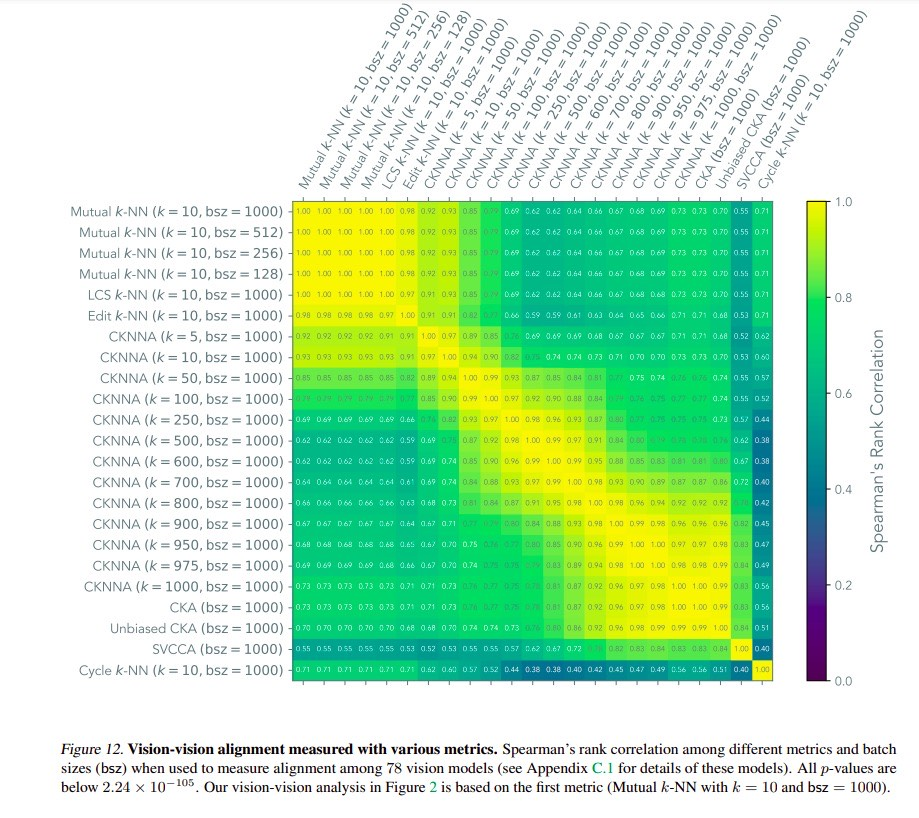
\includegraphics[width=\textwidth]{prh_correlation.jpg}
    \caption{Spearman rank correlation between models on Places365's validation data, indicating a high degree of alignment in in-distribution data.}
    \label{fig:prh_correlation}
\end{figure}

\subsection{Alignment on ImageNet-O Data}
\begin{figure}[H]
    \centering
    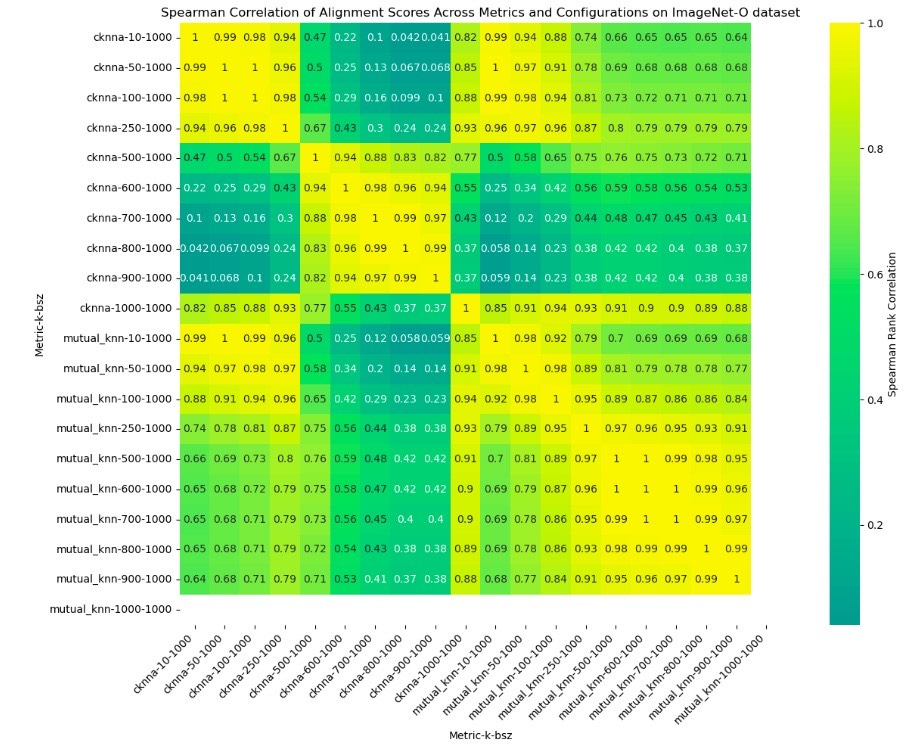
\includegraphics[width=\textwidth]{prh_correlation_ood.jpg}
    \caption{Alignment of vision models on the ImageNet-O dataset. The Spearman correlation suggests that even with outlier data, models maintain a shared statistical representation, albeit with higher prediction errors.}
    \label{fig:prh_correlation_ood}
\end{figure}

\textit{[Placeholder: Provide a detailed analysis of these results. What does this alignment imply about the robustness of PRH in OOD settings?]}

\subsection{Alignment on Random Noise Data}
\begin{figure}[H]
    \centering
    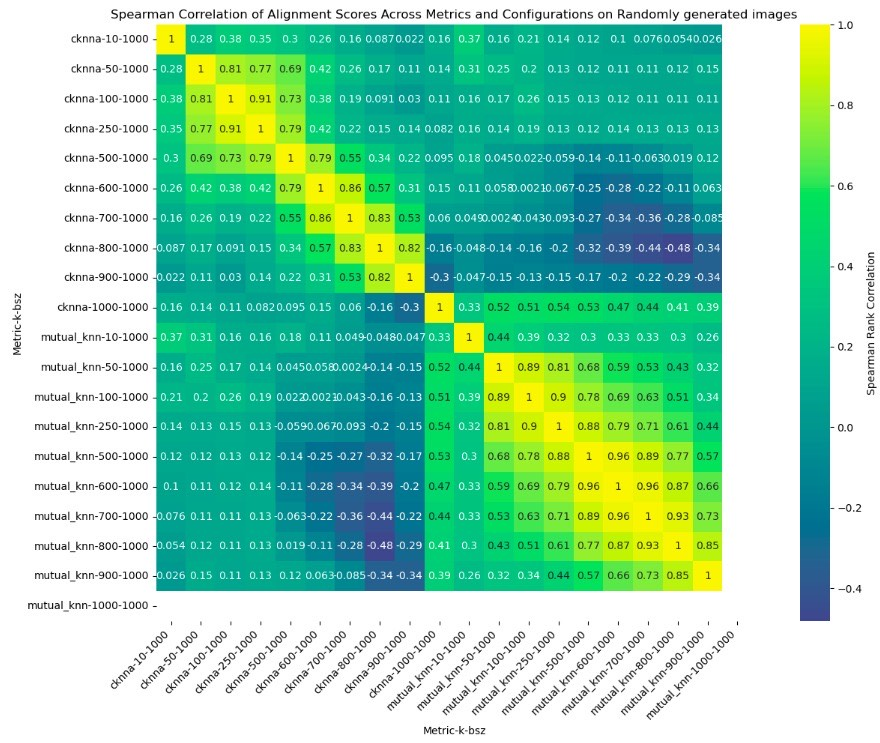
\includegraphics[width=\textwidth]{prh_correlation_random.jpg}
    \caption{Spearman correlation of alignment scores on random noise data. The lower correlation values indicate a breakdown in representational alignment, suggesting that random data lacks the underlying structure needed for PRH.}
    \label{fig:prh_correlation_random}
\end{figure}

\textit{[Placeholder: Discuss why PRH breaks down with random noise. Include insights into how this contrasts with the OOD findings and implications for the limits of representational alignment.]}

\subsection{Impact of Noise Injection}
\begin{figure}[H]
    \centering
    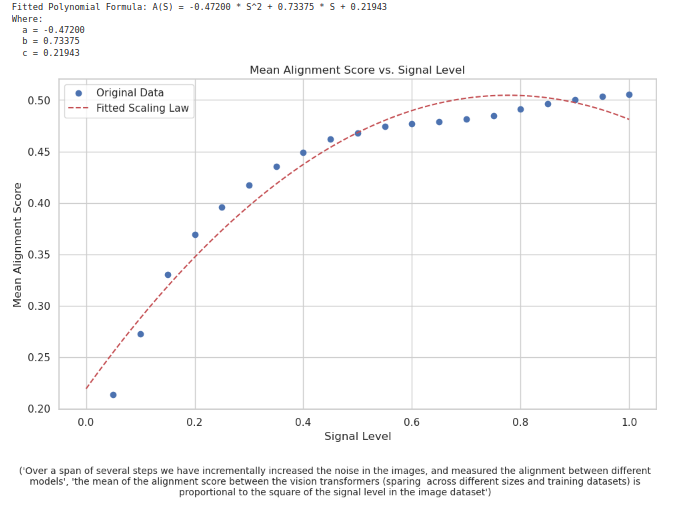
\includegraphics[width=\textwidth]{alignment_vs_signal_level.png}
    \caption{Relationship between noise level and mean alignment scores of 17 ViT models. A quadratic trend is observed as noise increases.}
    \label{fig:alignment_vs_signal_level}
\end{figure}

\textit{[Placeholder: Provide a mathematical explanation or hypothesis for the quadratic relationship. Discuss any exceptions or unexpected patterns observed.]}

\subsection{Alignment Dynamics During LLM Training}
\begin{figure}[H]
    \centering
    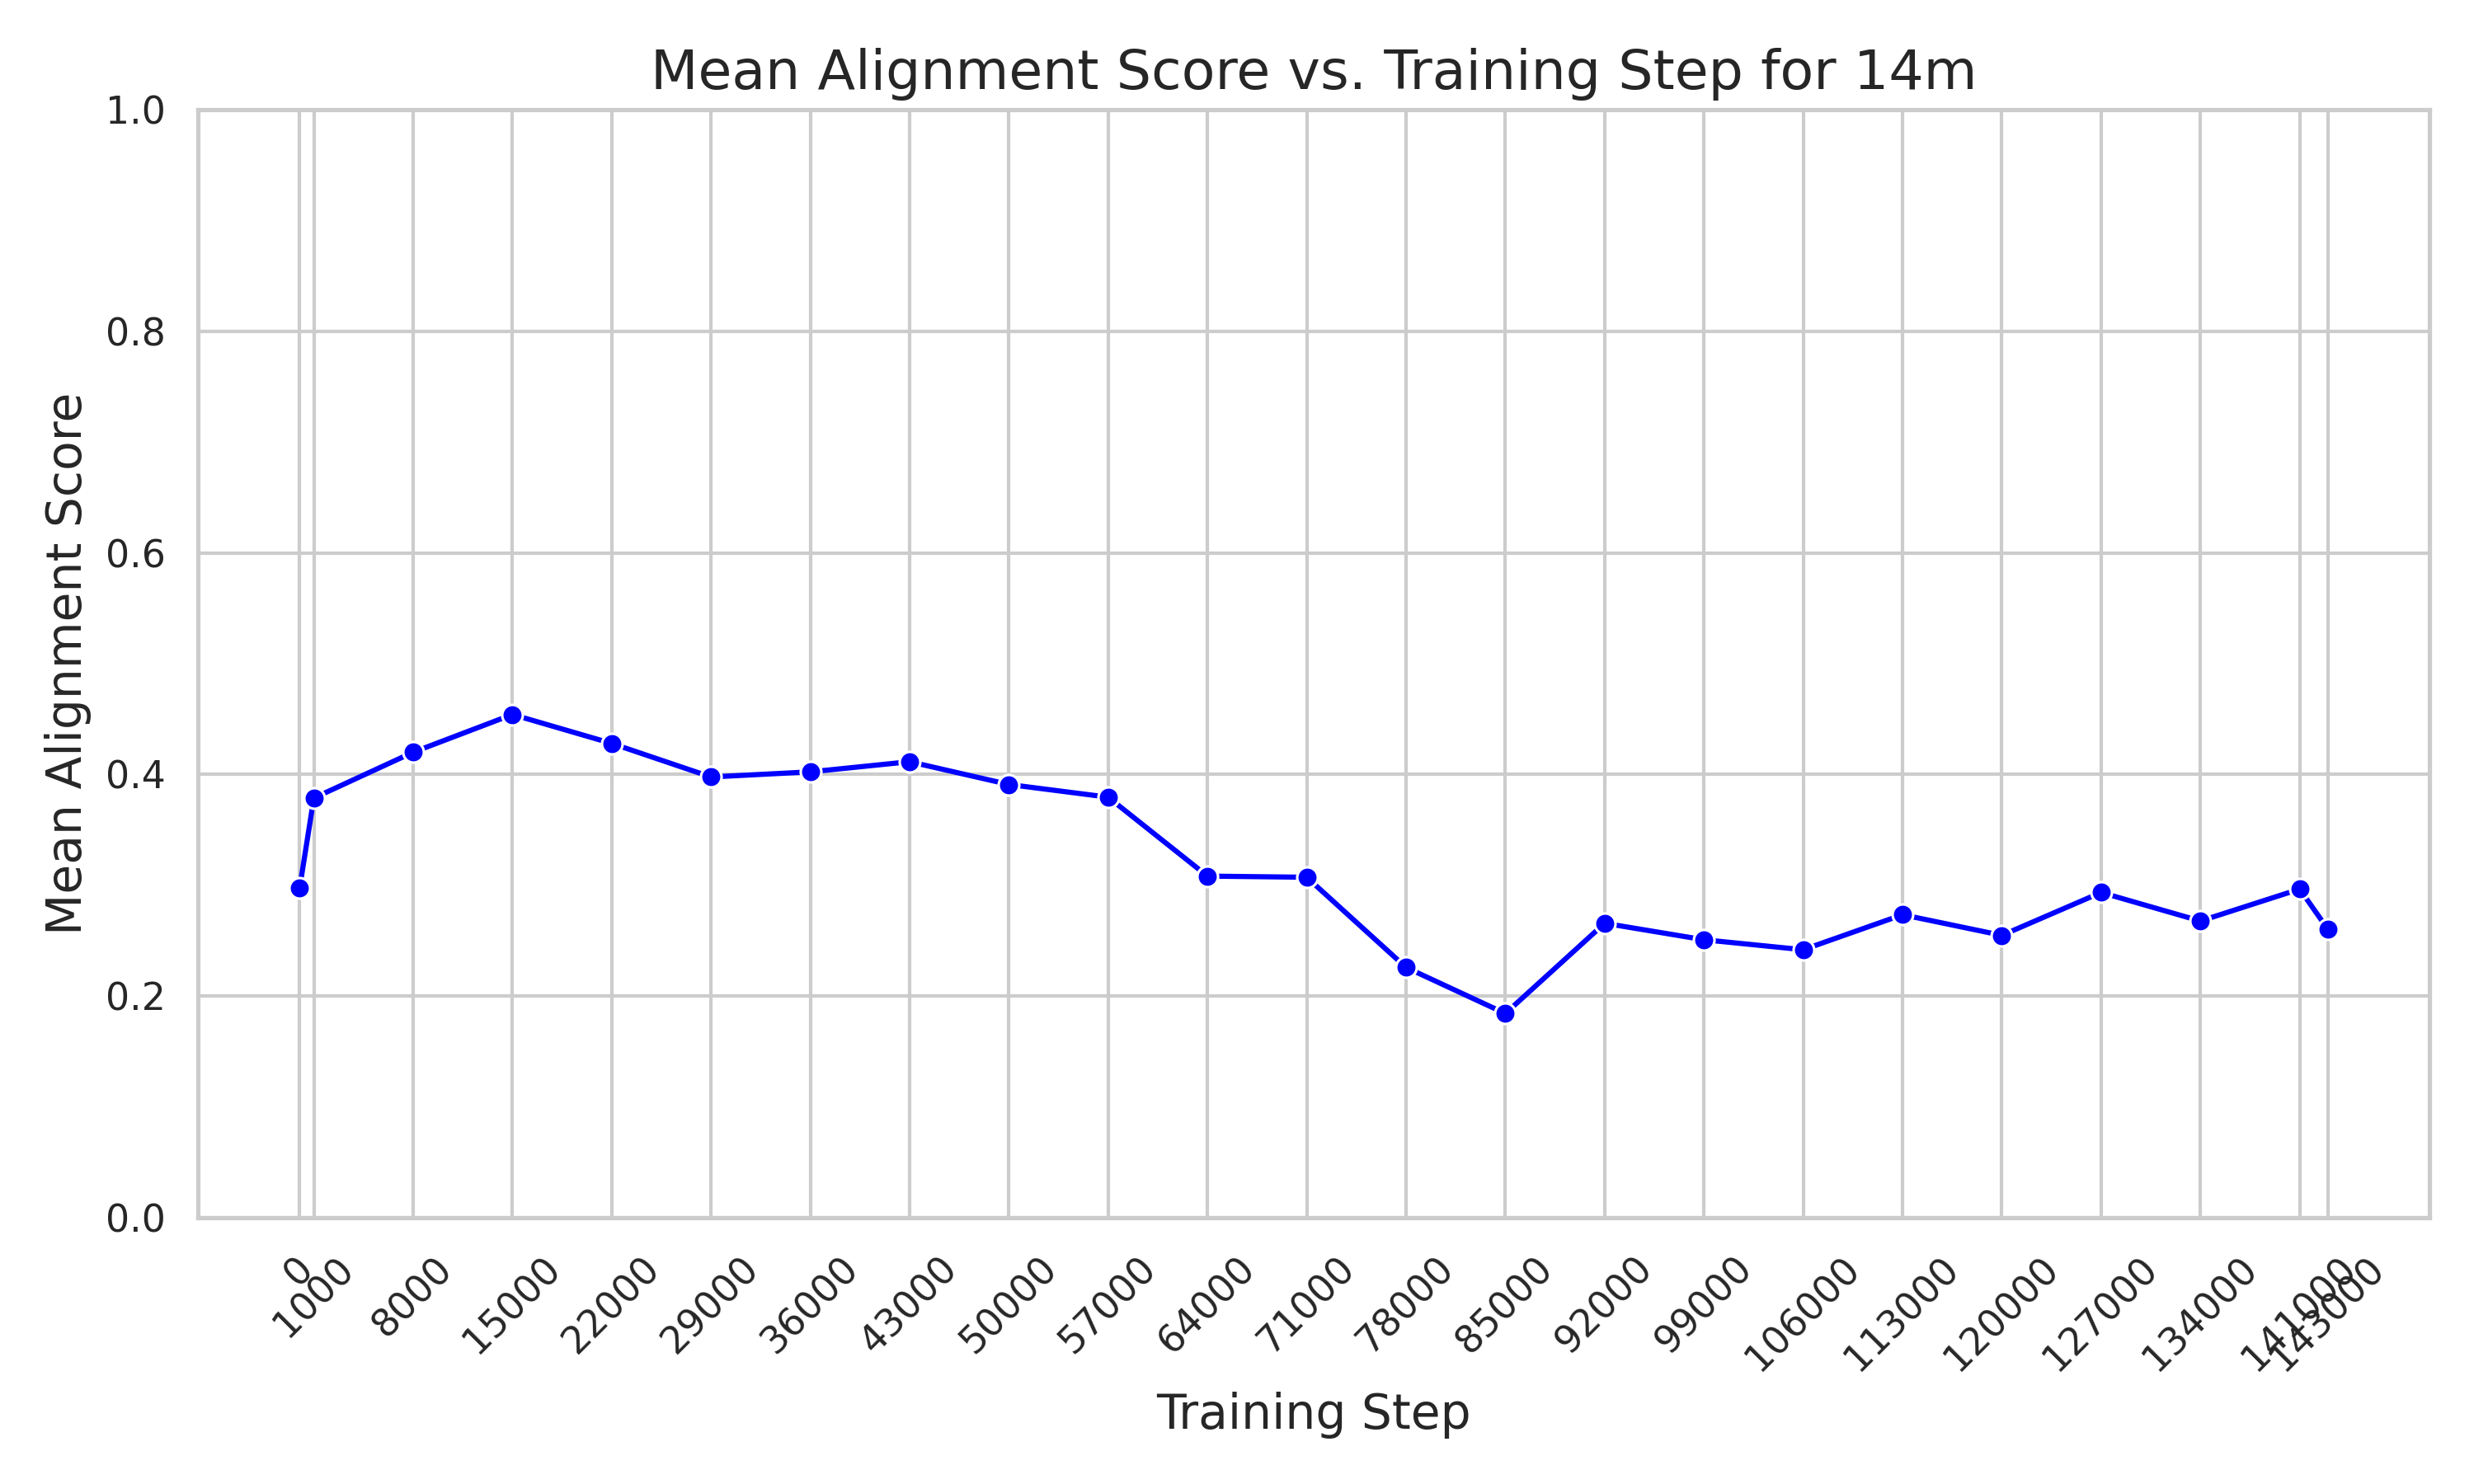
\includegraphics[width=0.48\textwidth]{mean_alignment_score_14m.png}
    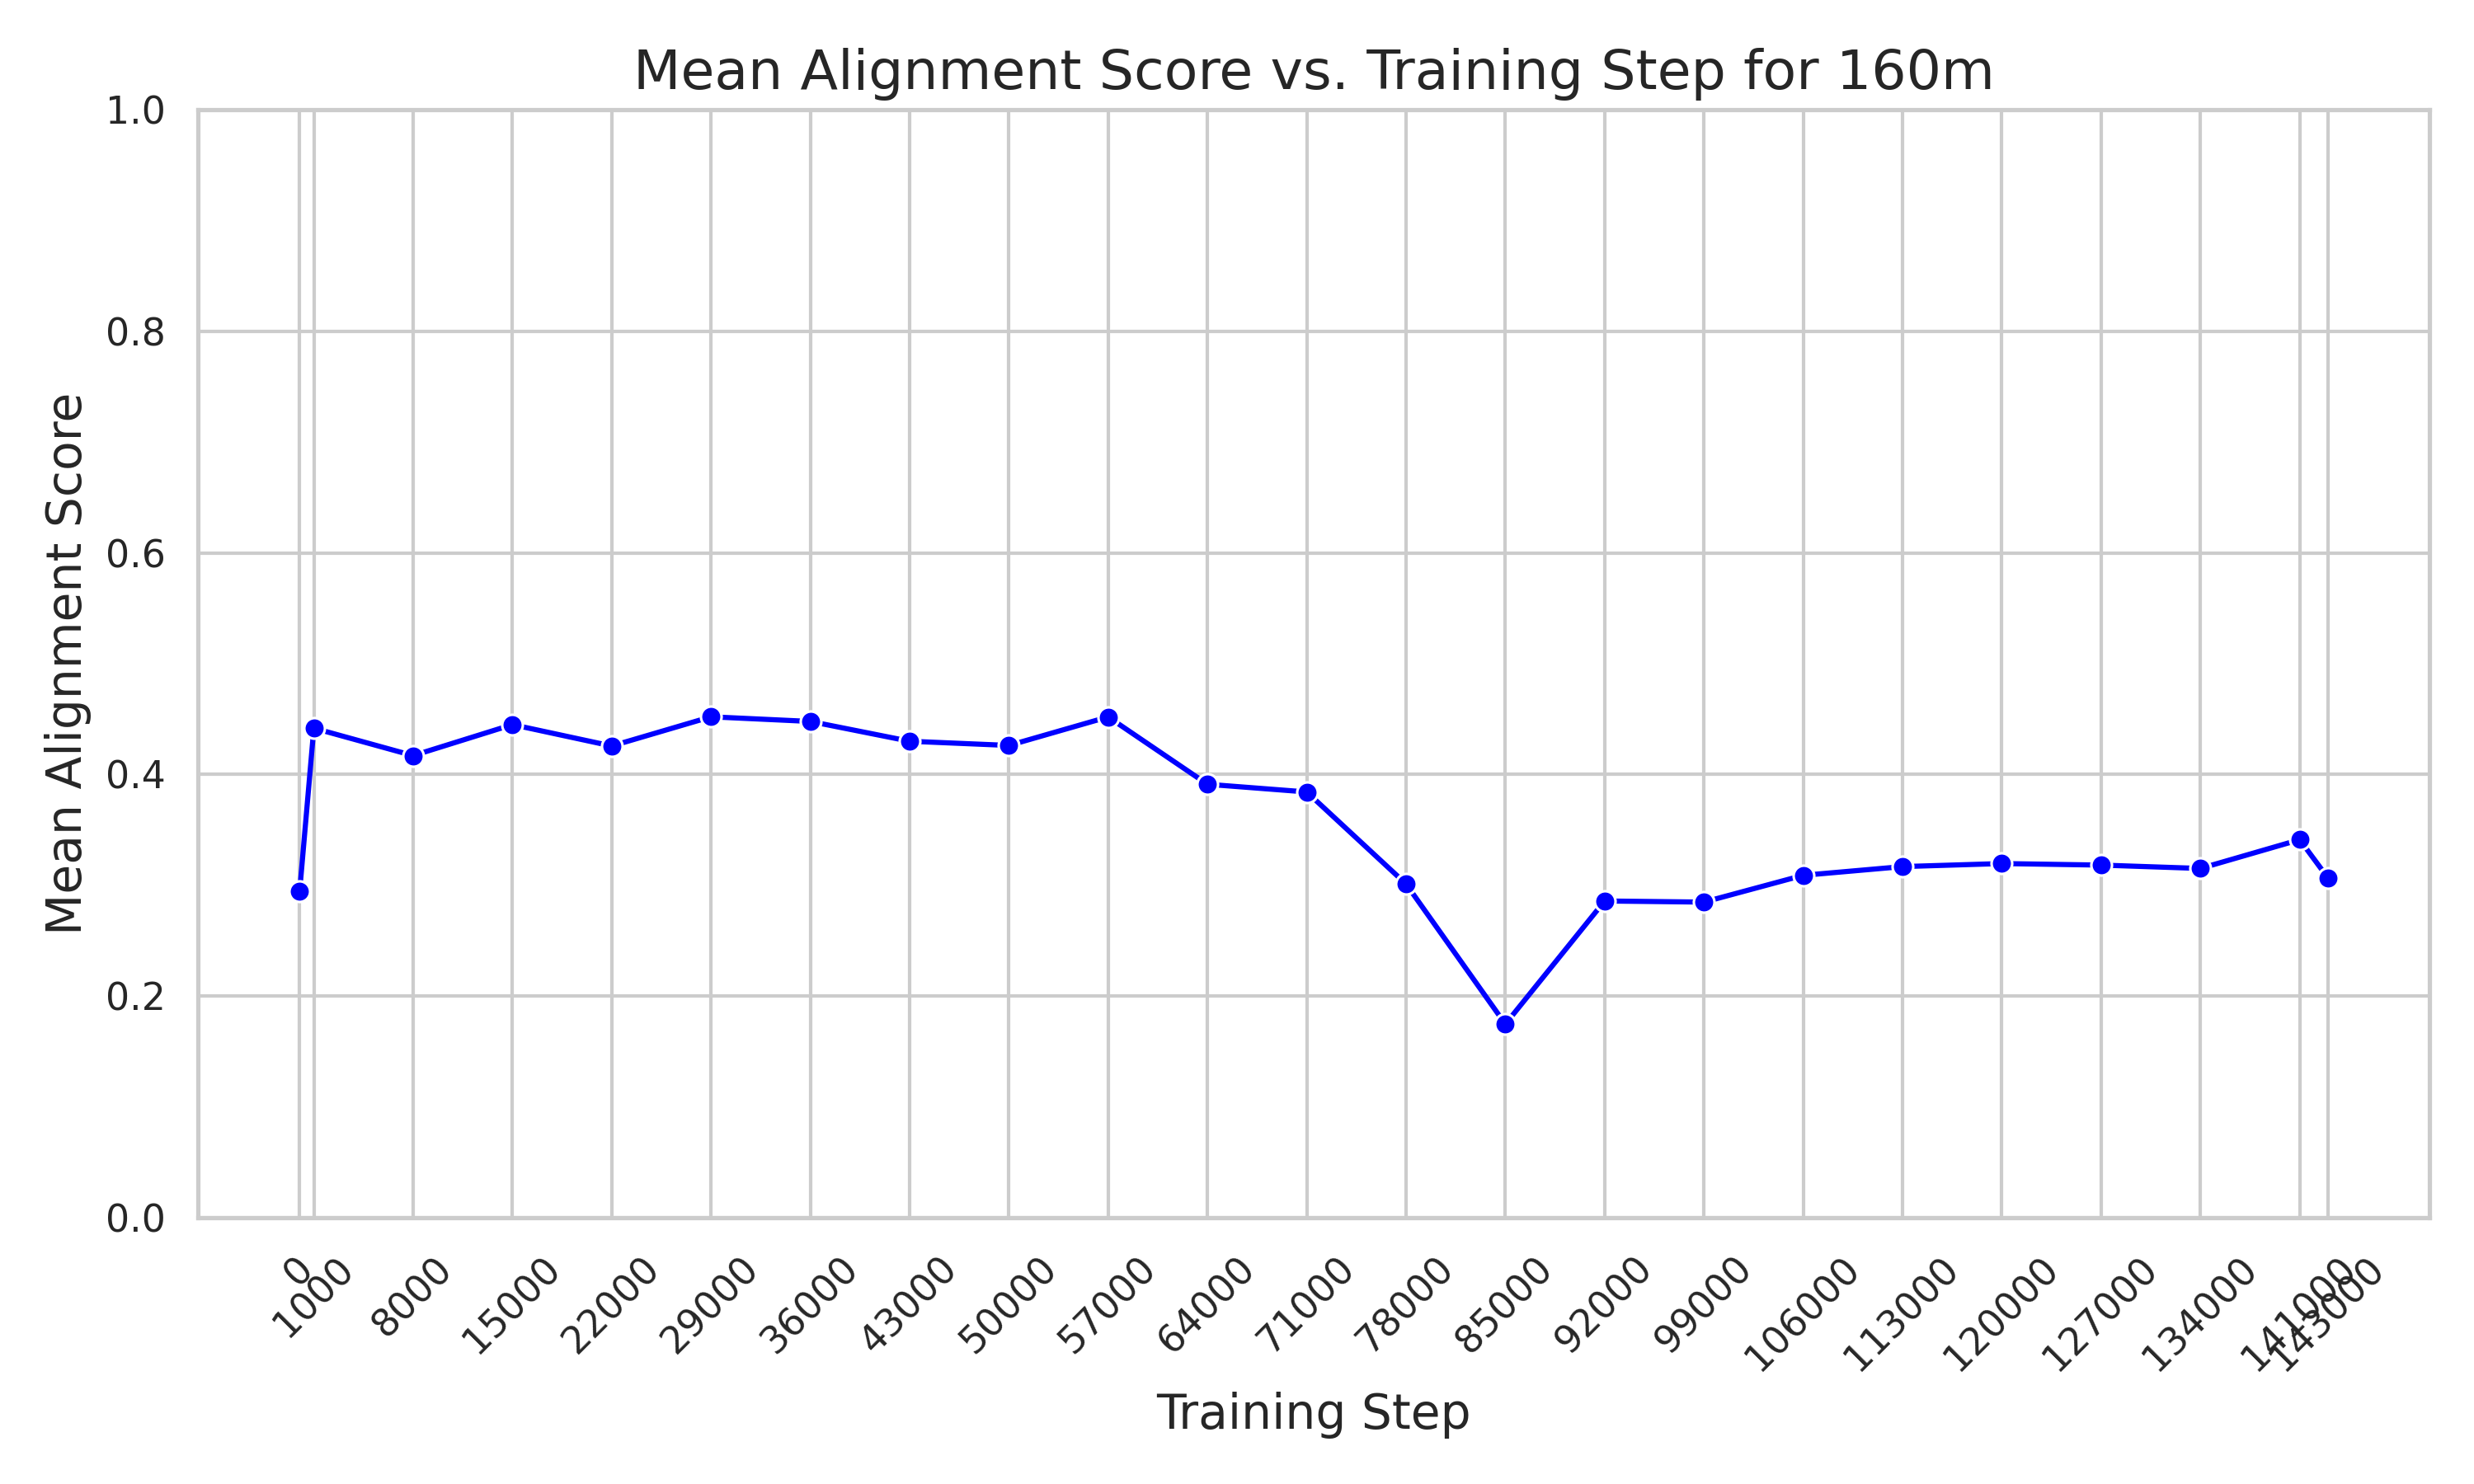
\includegraphics[width=0.48\textwidth]{mean_alignment_score_160m.png}
    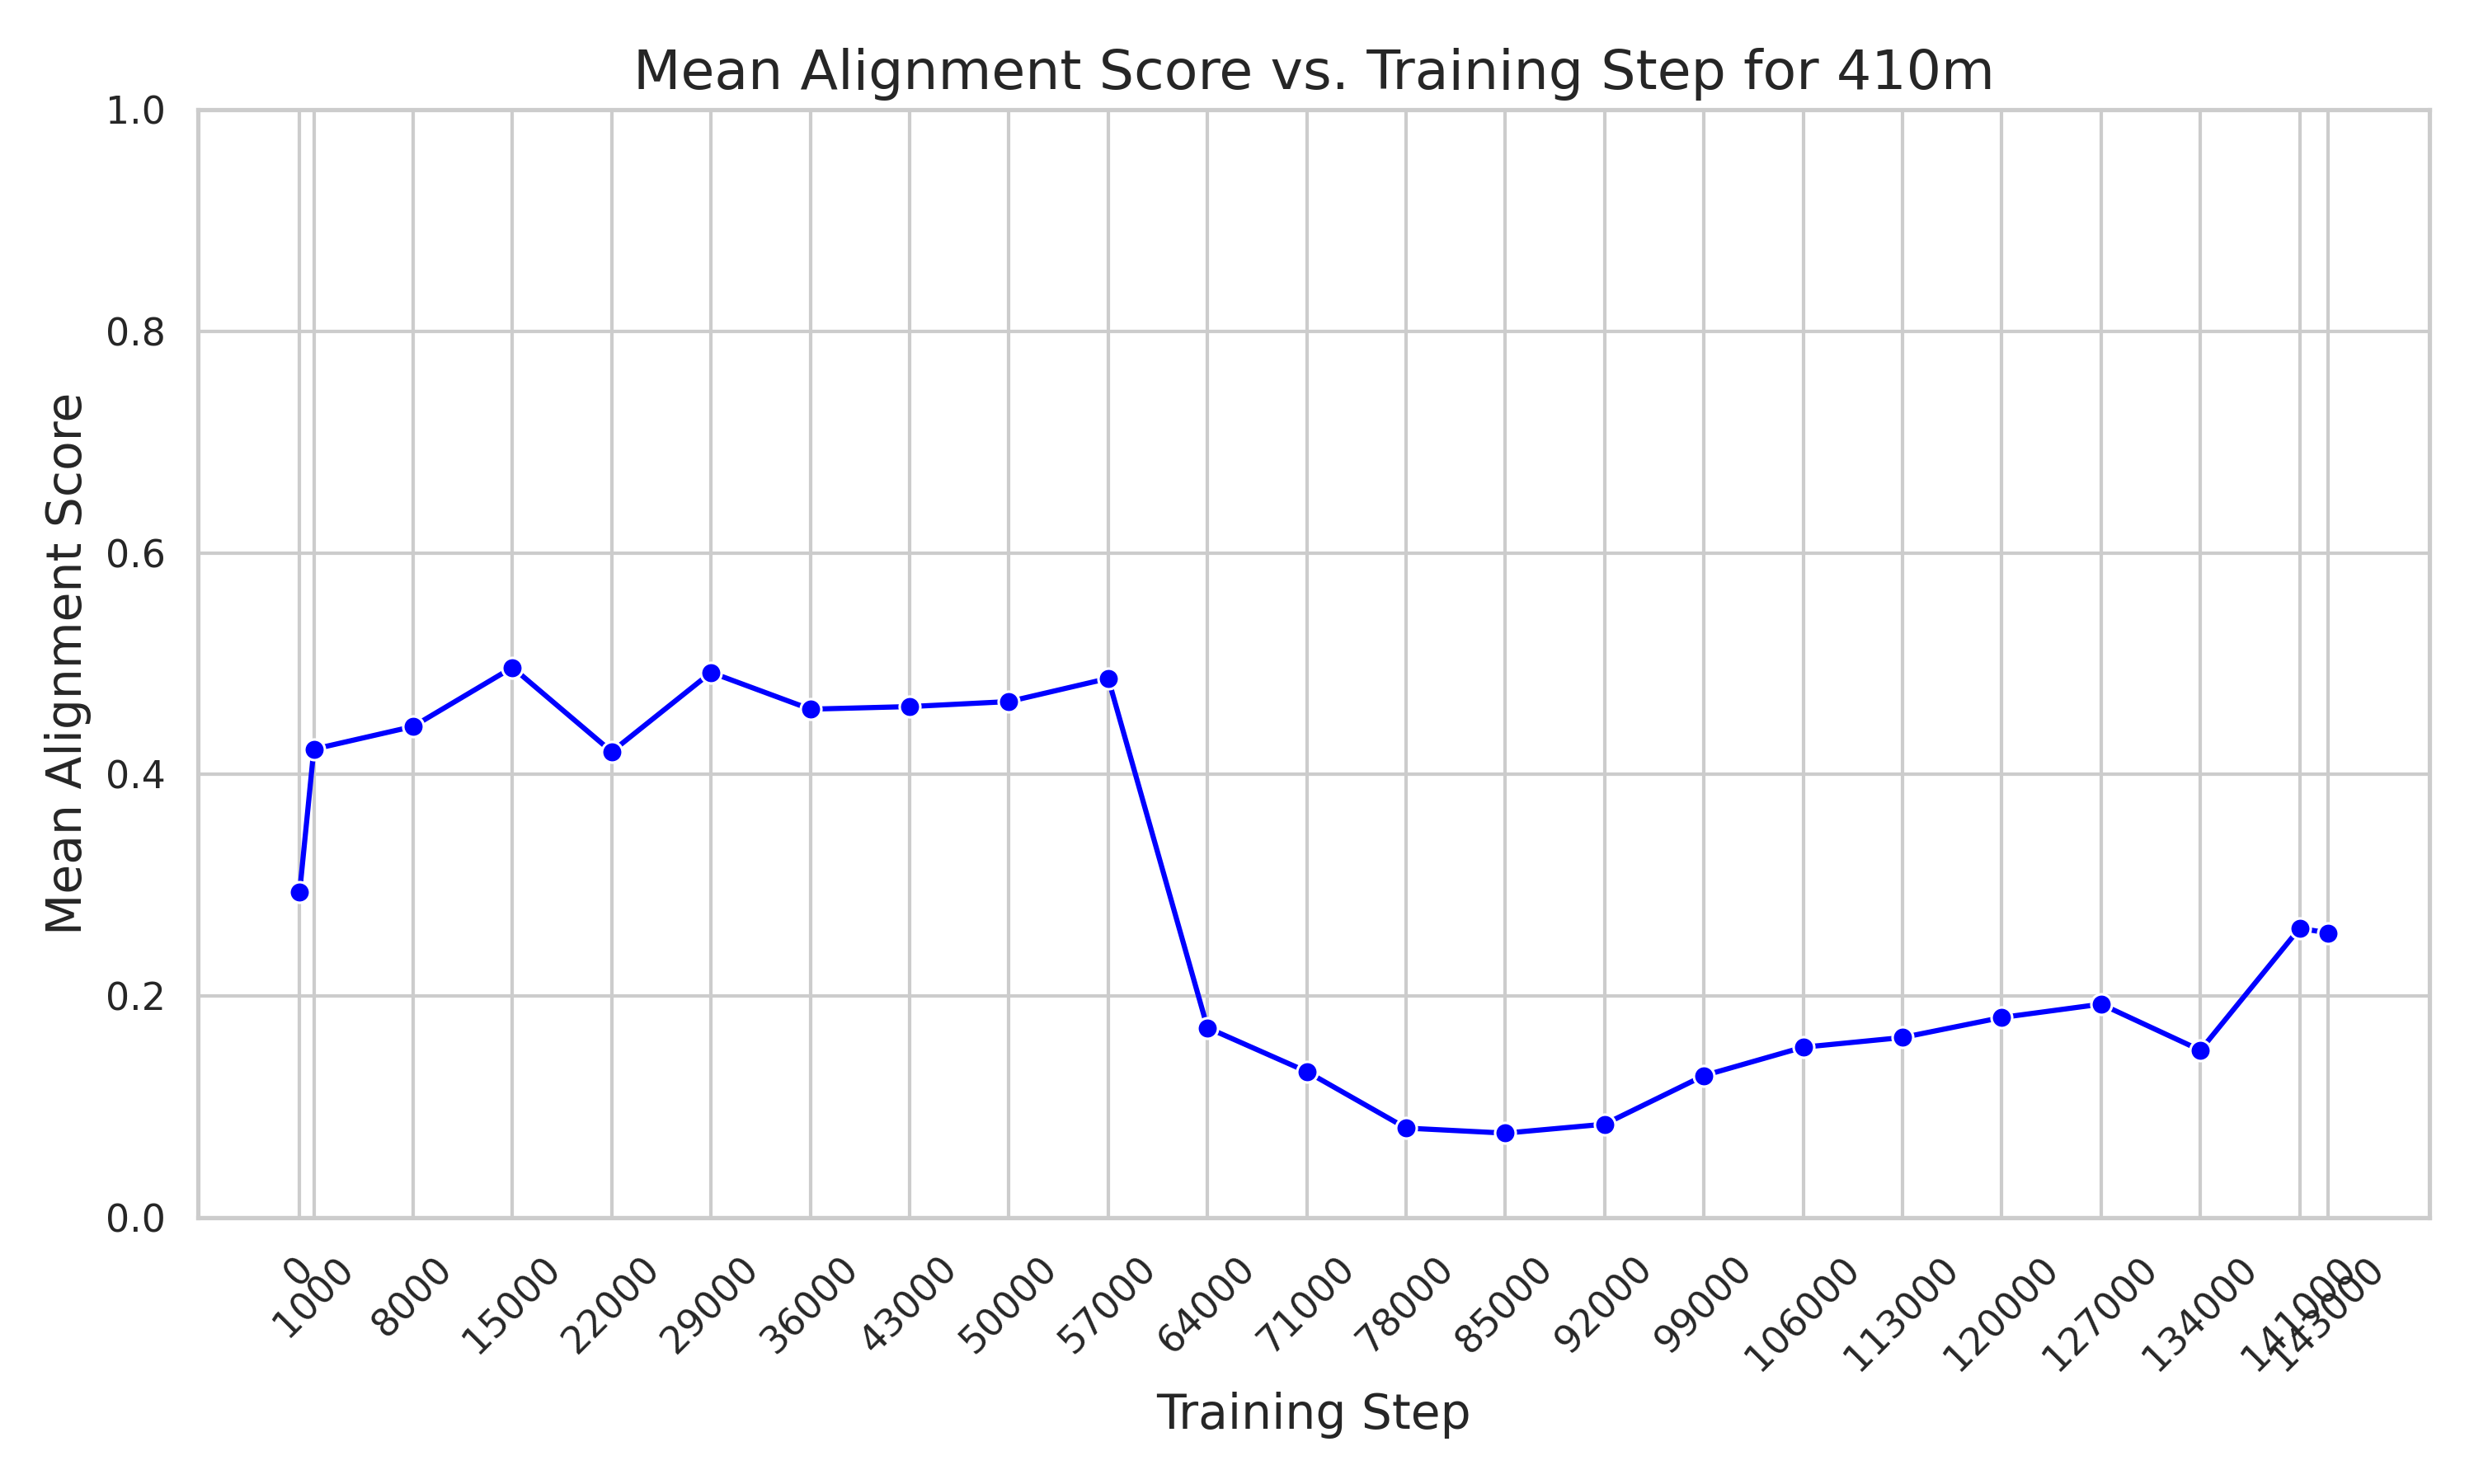
\includegraphics[width=0.48\textwidth]{mean_alignment_score_410m.png}
    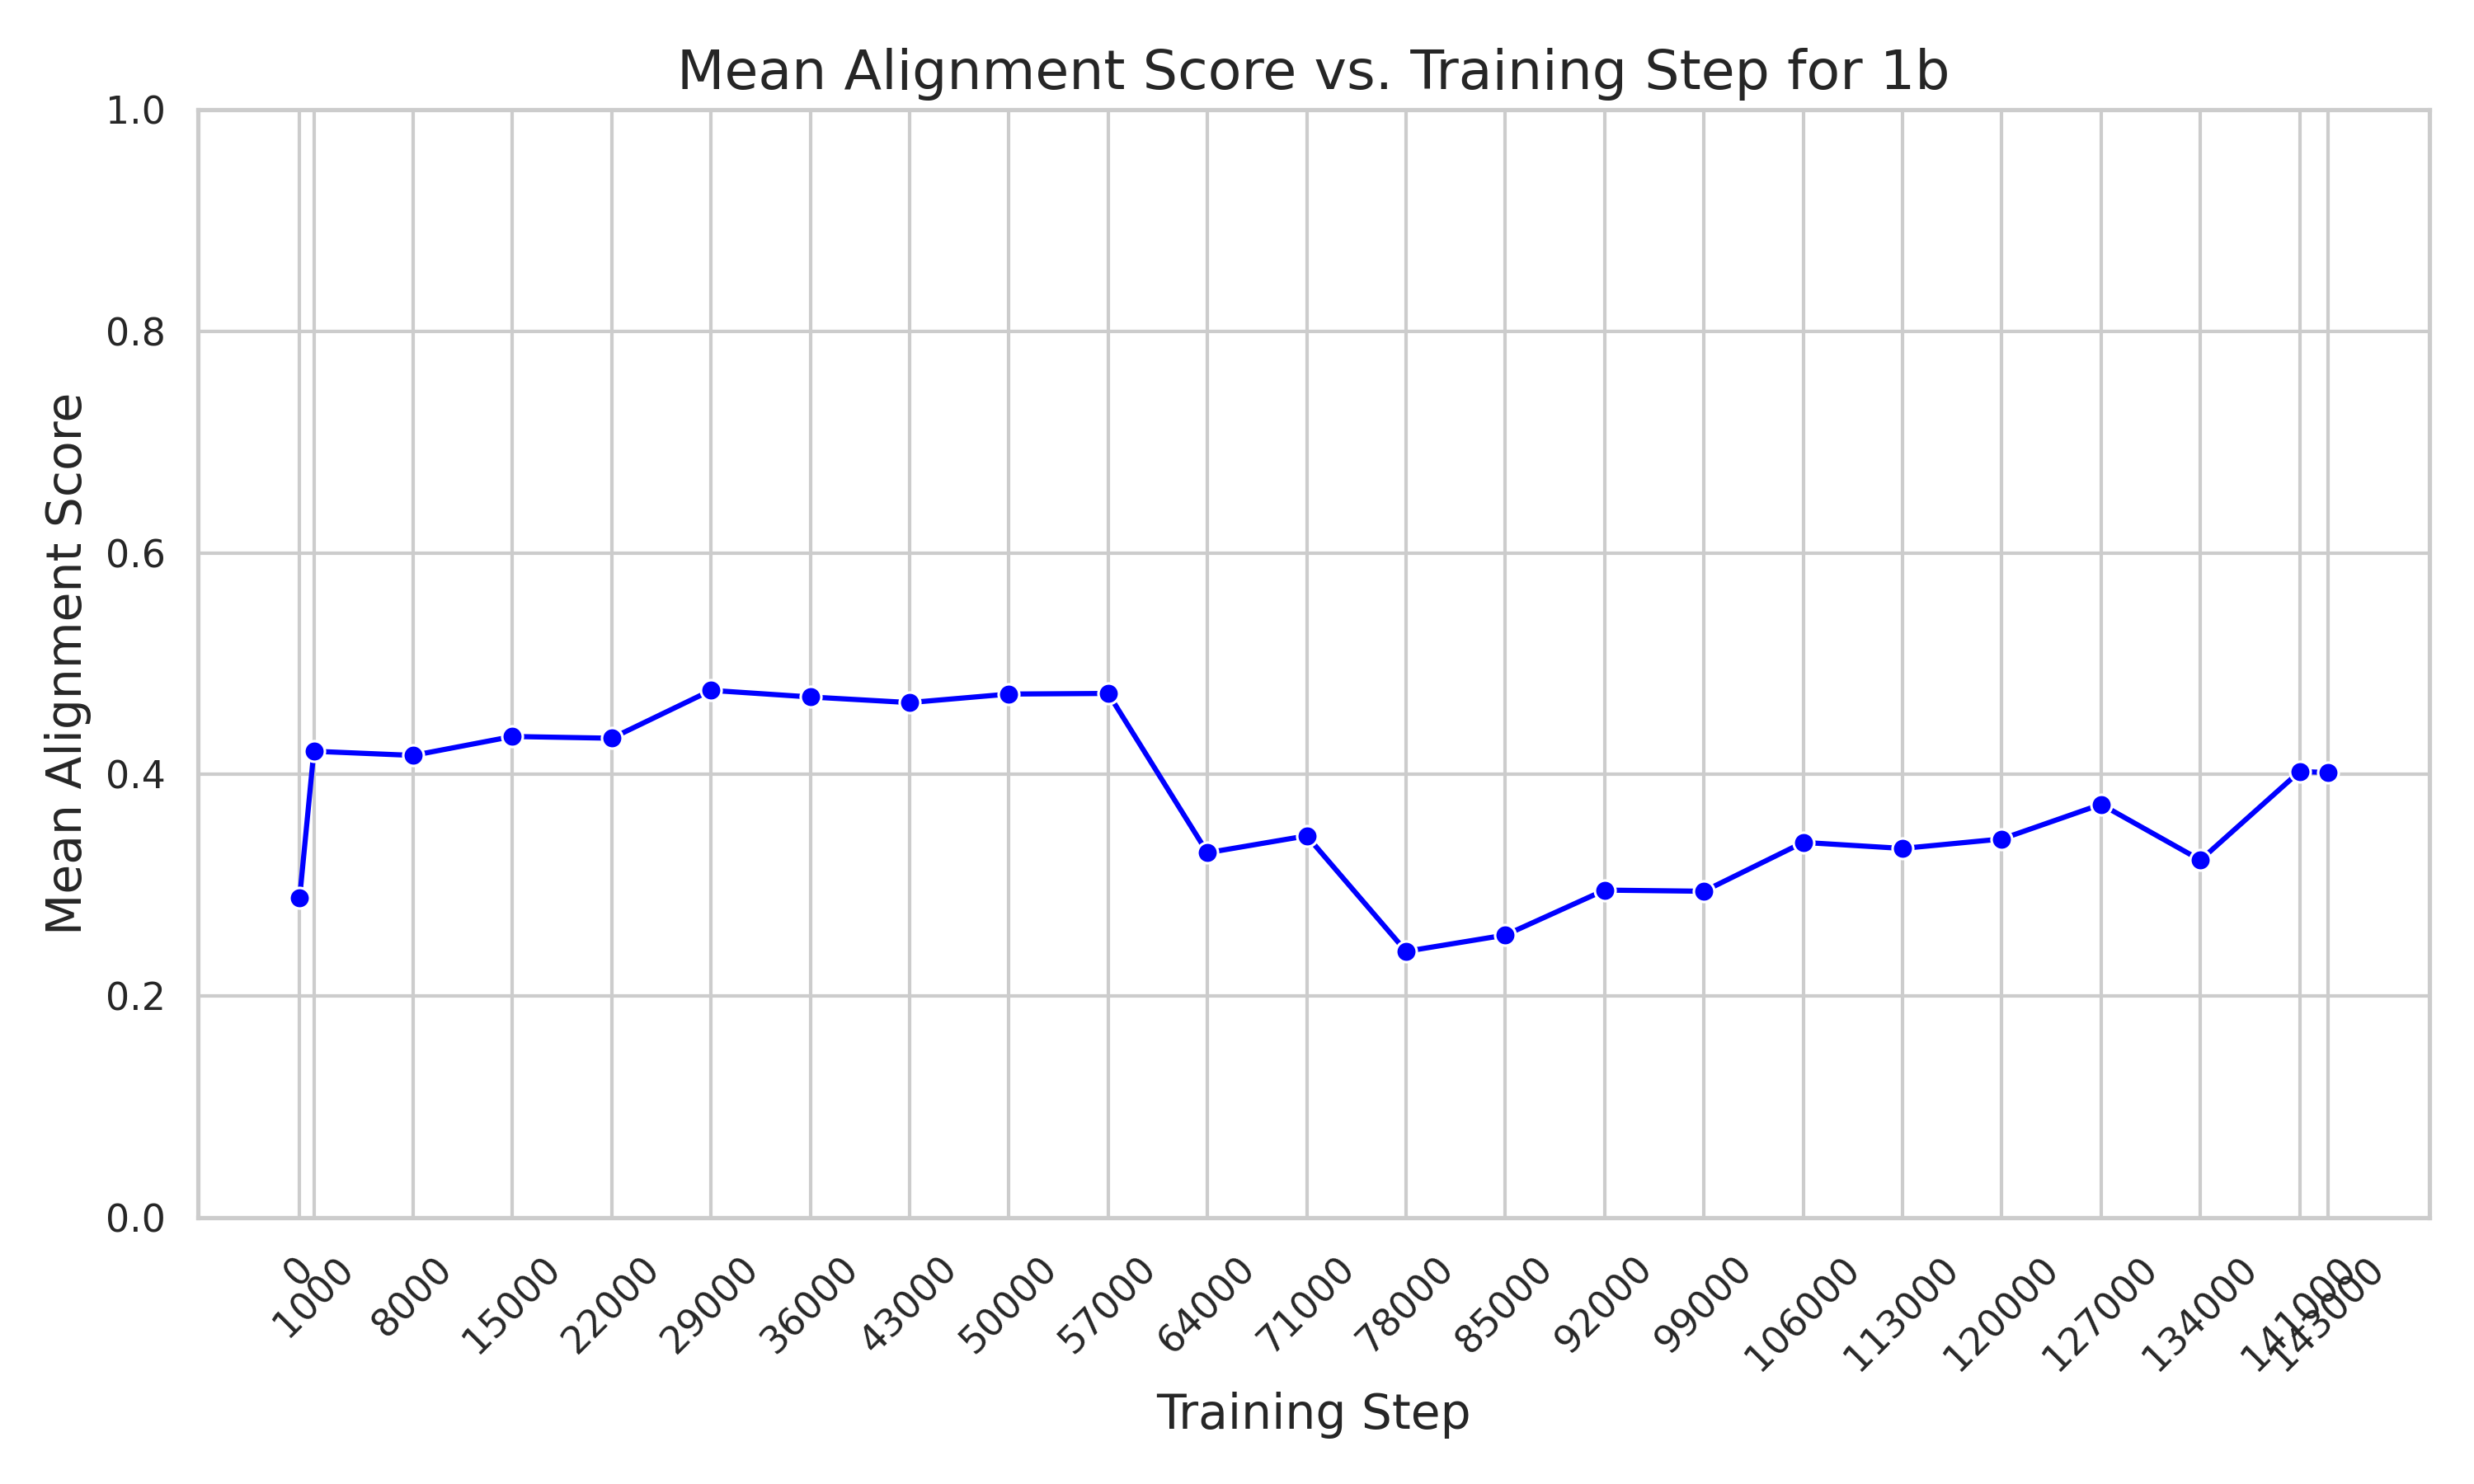
\includegraphics[width=0.48\textwidth]{mean_alignment_score_1b.png}
    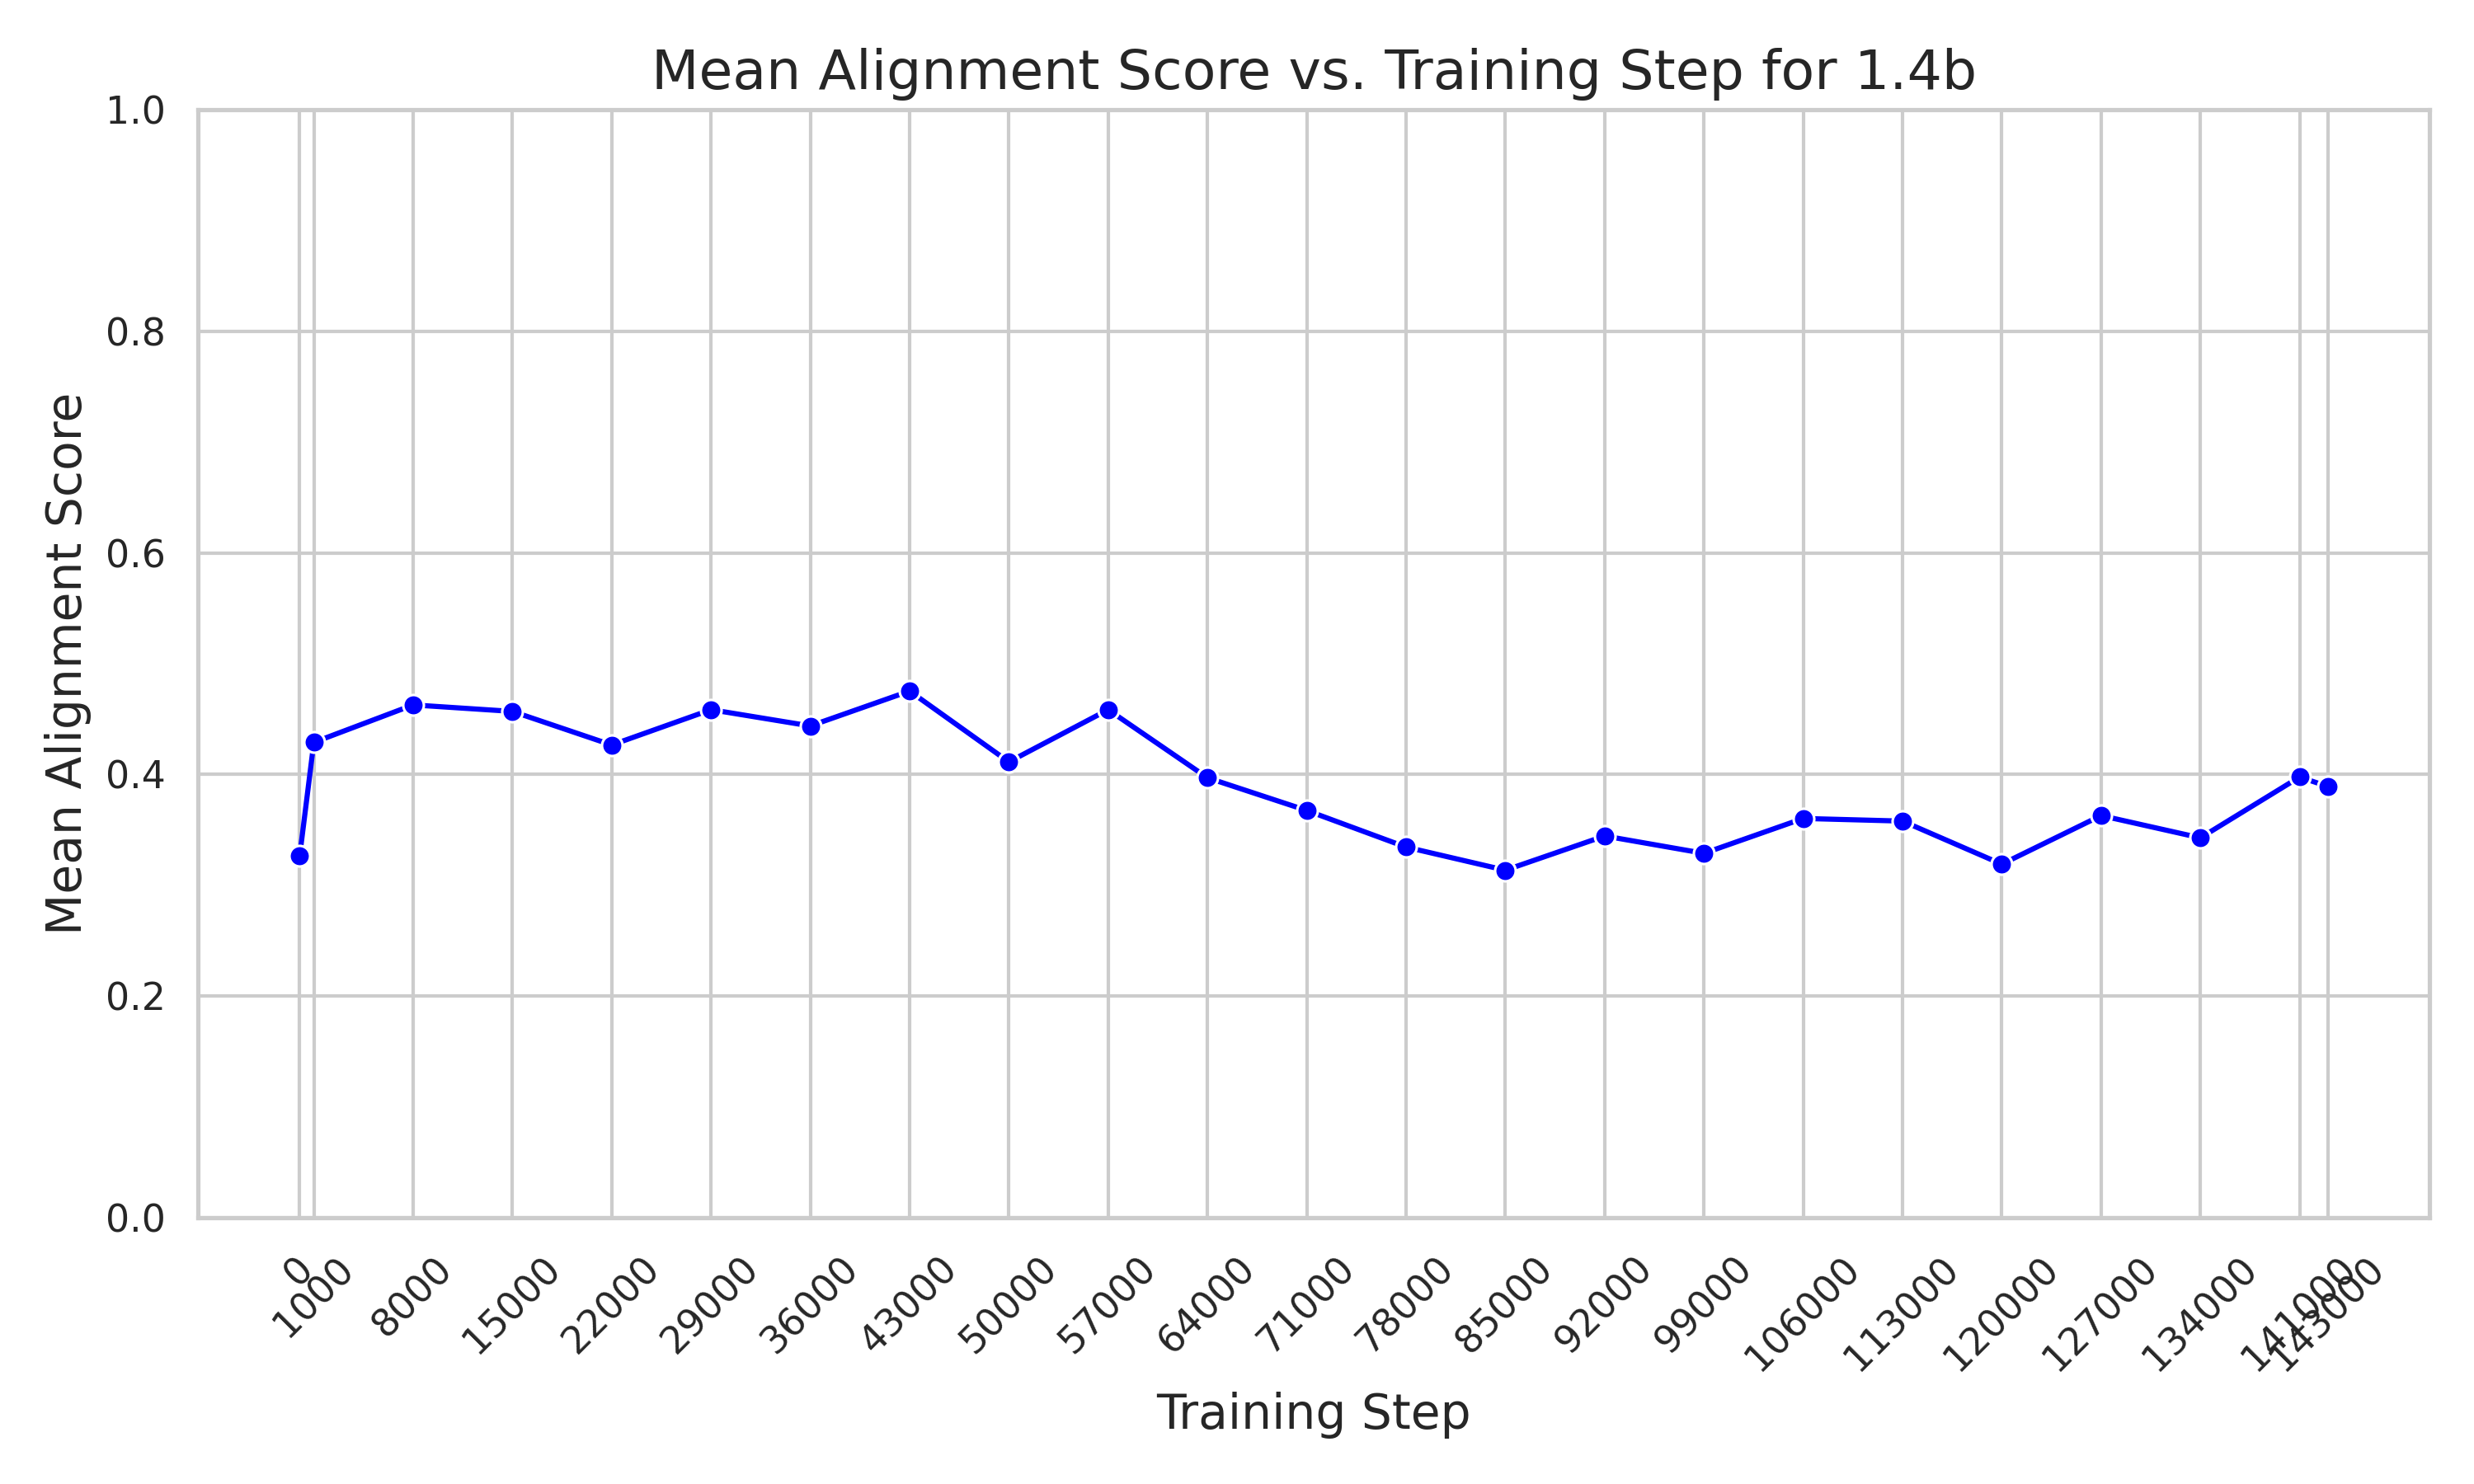
\includegraphics[width=0.48\textwidth]{mean_alignment_score_1.4b.png}
    \caption{Alignment trends of LLMs during training. Alignment scores reveal non-linear trends across different parameter sizes.}
    \label{fig:llm_training_alignment}
\end{figure}

\textit{[Placeholder: Discuss potential reasons for the observed non-linear trends. Do these trends correlate with known phases in model training, such as learning rate schedules or architectural changes?]}

\section{Discussion}
Our results extend the understanding of PRH by demonstrating that while neural networks maintain representational alignment in OOD settings, they struggle with random, unstructured data. This suggests that the shared statistical model proposed by PRH is dependent on the presence of underlying structures in the input data.

The resilience of model alignment to noise, as seen in our noise injection experiment, indicates a form of robustness in how models interpret degraded input. However, the breakdown of alignment with random noise raises questions about the limits of shared representations.

\textit{[Placeholder: Reflect on how these findings challenge or support the philosophical basis of PRH. Include thoughts on how future research could build on these observations.]}

\section{Conclusion}
Our study supports the validity of the Platonic Representation Hypothesis in structured, yet diverse data environments. The findings emphasize the importance of structured data for achieving alignment and suggest further exploration into the dynamics of alignment during model training. Future work could focus on extending PRH to multimodal settings and investigating the impact of training strategies on representational convergence.

\vfill
The code used for the experiments and analysis in this paper is available on GitHub \href{https://github.com/rokosbasilisk/prh-experiments}{here}.

\clearpage
\begin{thebibliography}{9}

\bibitem{huh2024prh}
Huh, M., Cheung, B., Wang, T., \& Isola, P. (2024). The Platonic Representation Hypothesis. \emph{International Conference on Machine Learning}.

\bibitem{hendrycks2021nae}
Hendrycks, D., Zhao, K., Basart, S., Steinhardt, J., \& Song, D. (2021). Natural Adversarial Examples. \emph{CVPR}. \href{https://arxiv.org/abs/2405.07987}{arXiv:2405.07987}.

\end{thebibliography}

\end{document}

